\chapter{Einleitung}
\label{ch:einleitung}
\Autor{Christopher Kroll}\\ \\
Im Master-Studiengang Informatik an der Universit"at Hamburg ist ein zweisemestriges Projekt vorgesehen. Die Autoren dieser Arbeit belegten im Sommersemester 2012 und Wintersemester 2012/2013 das Projekt 'Bildverarbeitung' unter der Leitung von Prof. Dr. Leonie Dreschler-Fischer. \\
Der Verlauf und das Ergebnis dieses Projektes wird in dem vorliegenden Dokument dargestellt.
\\ \\
Die Studenten sollten in diesem Projekt die Daten der Microsoft Kinect-Kamera nutzen und diese f"ur ein Thema ihrer Wahl verarbeiten. Nach einer Vorstellung der Kinect und der Programmiersprache Python wurden die Gruppen eingeteilt und das Thema gew"ahlt (siehe Kapitel \ref{aufgabenstellung} ).  \\ \\
Die digitale Bildverarbeitung hilft unter anderem bei der Erkennung von Objekten, wie zum Beispiel bei der vollautomatisierten Qualit"atskontrolle. Um auch bei gro"sen Datenmengen noch performant arbeiten zu k"onnen, bedient man sich oft des Mittels der Abstraktion. Das Projektthema dieser Arbeit dreht sich um eine M"oglichkeit der Abstraktion, n"amlich der Skelettierung. \\ \\
Der Begriff 'Skelett' taucht in vielen Fachbereichen, wie zum Beispiel der Anatomie, Biologie oder Architektur auf. In der digitalen Bildverarbeitung hat er einen "ahnlichen Sinn wie in diesen Bereichen: Es stellt von einem Objekt das Grundger"ust dar. Dieses Ger"ust ist der zentrale Hauptbestandteil, mit dessen Hilfe sich R"uckschl"usse auf das gesamte Objekt (zum Beispiel bei Dinosaurierskeletten) ergeben. \\ \\
Aus Sicht der Bildverarbeitung kann ein Skelett folgenderma"sen definiert werden: Ein Skelett ist ein n"utzlicher Deskriptor, um Informationen "uber die Region und den Rand eines Objektes kompakt und effizient zu kodieren und gibt die wesentlichen Grundz"uge eines Objektes wieder. In diesem Fachbereich kommen noch weitere Eigenschaften des Skeletts hinzu. Das Ziel ist die Information eines Objektes zu reduzieren ohne dabei die Grundstruktur zu verletzen. So ist eine Anforderung, dass die 'Pixelkonnektivit"at' gew"ahrleistet ist, also alle sp"ateren Skelettpixel mindestens einen benachbarten Skelettpixel besitzen und das Skelett nicht unterbrochen ist. \\ \\
Bei der Skelettierung muss weiterhin beachtet werden, dass die topologische Struktur des Originalbildes nicht ver"andert wird. Trotz eventueller Verformung bei der Skelettbildung, wie in Abbildung \ref{fig:topologischeStruktur} dargestellt, muss die strukturelle Eigenschaft erhalten bleiben; so ist bei einer automatisierten Zeichenerkennung die Strichst"arke unerheblich, lediglich der generelle Aufbau des Buchstaben ist relevant \cite{buhlmann}. \\
%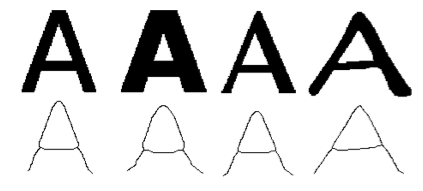
\includegraphics[width=1.0\linewidth]{./fig/topologischeStruktur}
\begin{figure}
\centering
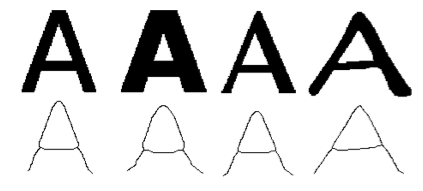
\includegraphics[width=0.7\linewidth]{./fig/topologischeStruktur}
\caption{Skelettierung des Buchstaben 'A'. Bildquelle:  \cite{buhlmann}}
\label{fig:topologischeStruktur}
\end{figure}


Um nun ein Skelett zu erhalten, gibt es verschiedene Ans"atze, die sich nach Art der Bestimmung der Skelettpunkte unterscheiden. Die meisten k"onnen in eine von drei Kategorien eingeteilt werden: Das Thinning (Ausd"unnen), die Distanztranformation und der kritische Punkte Ansatz. N"aheres zu den einzelnen Kategorien wird in Kapitel 3 beschrieben.


\section{Aufgabenstellung}
\label{aufgabenstellung}
Unsere Gruppe entschied sich f"ur die Datenauswertung einer Person ('Spieler'). Dabei war zun"achst das Ziel den Bewegungsablauf bei Sport"ubungen zu analysieren und eine R"uckmeldung zu geben, ob diese richtig ausgef"uhrt wurden. So soll zum Beispiel bei Kniebeugen durch eine Messung des Winkels zwischen Ober- und Unterschenkel der Person eine Hilfestellung gegeben werden. \\ \\ 
Um dieses Ziel zu erreichen muss zun"achst der Spieler von anderen Gegenst"anden im Raum getrennt, also herausgefiltert werden (Segmentierung). F"ur die Bewegungsanalyse ist es hilfreich nicht den gesamten Menschen, wom"oglich noch mit st"orender Kleidung, zu betrachten, sondern nur sein Skelett. Um das Skelett zu erhalten, bot sich die Wahl zwischen schon implementierten Skelettierungsalgorithmen zu benutzen oder dies selbst zu implementieren. Da das Thema des Projektes die Bildverarbeitung und nicht eine Anwendungsprogrammierung ist, fiel die Entscheidung auf die Konzentration auf die Skelettierung. Das Ziel war nun verschiedene Ans"atze zu implementieren und hinsichtlich Qualit"at und Leistung zu vergleichen.  \\ \\
Dabei mussten einige Kriterien beachtet werden. Zuallererst muss auf die Qualit"at des erzeugten Skeletts geachtet werden. Es sollte als eine Skelettrepr"asentation des Quellbildes erkannt werden, also ein zentrales Grundger"ust mit vorhandener Pixelkonnektivit"at. Desweiteren ist die Leistungsf"ahigkeit relevant. Die Algorithmen sollen echtzeitf"ahig sein, damit der Spieler eine unmittelbare R"uckmeldung seiner Bewegungen erh"alt.
\section{Aufbau der Projektarbeit}
Nach dieser Einleitung wird in Kapitel 2 die Microsoft Kinect-Kamera vorgestellt. Ihre einzelnen Komponenten werden beschrieben und Vor- und Nachteile der Kamera dargestellt. \\  \\ In Kapitel 3 wird n"aher auf die Skelettierung eingegangen, indem die Grundidee ausgef"uhrt und verschiedene Ans"atze zur Erzeugung eines Skeletts aufgezeigt werden. In den Unterkapiteln zu Thinning und Distanztransformation werden verwandte wissenschaftliche Arbeiten, mit denen sich im Seminarteil des Projektes besch"aftigt wurde, pr"asentiert. \\ \\ W"ahrend bis dahin eher die Theorie beleuchtet wurde, geht es im vierten Kapitel um die praktische Umsetzung: Das technische Umfeld, die Spielersegmentierung und die Umsetzung der beiden Skelettierungsmethoden werden hier vorgestellt. \\ \\ Kapitel 5 evaluiert die Umsetzung, indem die Skelettqualit"at und die Laufzeit der Algorithmen beleuchtet werden. Au"serdem werden hier "Uberlegungen zur Verbesserung gezeigt. \\ \\ Im abschlie"senden Kapitel 6 wird die gesamte Arbeit zusammengefasst und ein Ausblick, wie die Arbeit fortgef"uhrt werden kann, gegeben. \\ \\ Im Anhang befindet sich der Quellcode zu den erw"ahnenswerten Stellen der Implementation sowie eine Autoren"ubersicht zu den einzelnen Kapiteln, bzw. Abschnitten dieser Arbeit.